%% This is file `elsarticle-template-1-num.tex',
%%
%% Copyright 2009 Elsevier Ltd
%%
%% This file is part of the 'Elsarticle Bundle'.
%% ---------------------------------------------
%%
%% It may be distributed under the conditions of the LaTeX Project Public
%% License, either version 1.2 of this license or (at your option) any
%% later version.  The latest version of this license is in
%%    http://www.latex-project.org/lppl.txt
%% and version 1.2 or later is part of all distributions of LaTeX
%% version 1999/12/01 or later.
%%
%% The list of all files belonging to the 'Elsarticle Bundle' is
%% given in the file `manifest.txt'.
%%
%% Template article for Elsevier's document class `elsarticle'
%% with numbered style bibliographic references
%%
%% $Id: elsarticle-template-1-num.tex 149 2009-10-08 05:01:15Z rishi $
%% $URL: http://lenova.river-valley.com/svn/elsbst/trunk/elsarticle-template-1-num.tex $
%%

%\documentclass[preprint,authoryear,review,12pt]{elsarticle}
\documentclass[final,5p,times,twocolumn]{elsarticle}

%% Use the option review to obtain double line spacing
%% \documentclass[preprint,review,12pt]{elsarticle}

%% Use the options 1p,twocolumn; 3p; 3p,twocolumn; 5p; or 5p,twocolumn
%% for a journal layout:
%% \documentclass[final,1p,times]{elsarticle}
%% \documentclass[final,1p,times,twocolumn]{elsarticle}
%% \documentclass[final,3p,times]{elsarticle}
%% \documentclass[final,3p,times,twocolumn]{elsarticle}
%% \documentclass[final,5p,times]{elsarticle}
%% \documentclass[final,5p,times,twocolumn]{elsarticle}


\usepackage{color}
\usepackage{multirow,booktabs,ctable,array}
\usepackage{lscape}
\usepackage{amsmath}
\usepackage{lineno}
\usepackage{ulem}
\usepackage{setspace}
\usepackage{listings}
\usepackage{float}


\floatstyle{plain}
\newfloat{command}{thp}{lop}
\floatname{command}{Command}

%\usepackage[nomarkers,notablist]{endfloat}

%% if you use PostScript figures in your article
%% use the graphics package for simple commands
%% \usepackage{graphics}
%% or use the graphicx package for more complicated commands
%% \usepackage{graphicx}
%% or use the epsfig package if you prefer to use the old commands
%% \usepackage{epsfig}

%% The amssymb package provides various useful mathematical symbols
\usepackage{amssymb}
%% The amsthm package provides extended theorem environments
% \usepackage{amsthm}
 
 \usepackage{makecell}

%% The lineno packages adds line numbers. Start line numbering with
%% \begin{linenumbers}, end it with \end{linenumbers}. Or switch it on
%% for the whole article with \linenumbers after \end{frontmatter}.
%% \usepackage{lineno}

%% natbib.sty is loaded by default. However, natbib options can be
%% provided with \biboptions{...} command. Following options are
%% valid:

%%   round  -  round parentheses are used (default)
%%   square -  square brackets are used   [option]
%%   curly  -  curly braces are used      {option}
%%   angle  -  angle brackets are used    <option>
%%   semicolon  -  multiple citations separated by semi-colon
%%   colon  - same as semicolon, an earlier confusion
%%   comma  -  separated by comma
%%   numbers-  selects numerical citations
%%   super  -  numerical citations as superscripts
%%   sort   -  sorts multiple citations according to order in ref. list
%%   sort&compress   -  like sort, but also compresses numerical citations
%%   compress - compresses without sorting
%%
%% \biboptions{comma,round}

% \biboptions{}

\providecommand{\OO}[1]{\operatorname{O}\bigl(#1\bigr)}

\graphicspath{{./Figures/}
                          }

\long\def\symbolfootnote[#1]#2{\begingroup%
\def\thefootnote{\fnsymbol{footnote}}\footnote[#1]{#2}\endgroup}

    \usepackage{color}

    \definecolor{listcomment}{rgb}{0.0,0.5,0.0}
    \definecolor{listkeyword}{rgb}{0.0,0.0,0.5}
    \definecolor{listnumbers}{gray}{0.65}
    \definecolor{listlightgray}{gray}{0.955}
    \definecolor{listwhite}{gray}{1.0}

\newcommand{\lstsetcpp}
{
\lstset{frame = tb,
        framerule = 0.25pt,
        float,
        fontadjust,
        backgroundcolor={\color{listlightgray}},
        basicstyle = {\ttfamily\scriptsize},
        keywordstyle = {\ttfamily\color{listkeyword}\textbf},
        identifierstyle = {\ttfamily},
        commentstyle = {\ttfamily\color{listcomment}\textit},
        stringstyle = {\ttfamily},
        showstringspaces = false,
        showtabs = false,
        numbers = none,
        numbersep = 6pt,
        numberstyle={\ttfamily\color{listnumbers}},
        tabsize = 2,
        language=[ANSI]C++,
        floatplacement=!h,
        caption={},
        captionpos=b,
        }
}


\journal{Neuroimage}

\begin{document}


\begin{frontmatter}

\title{ANTs-Flavored Tract-Based Spatial Statistics}



\author[label1]{Nicholas J.~Tustison\fnref{label0}}
%  \ead{ntustison@virginia.edu}
  \fntext[label0]{\scriptsize Corresponding author:  PO Box 801339, Charlottesville, VA 22908; T:  434-924-7730; email address:  ntustison@virginia.edu }
\author[label2]{Brian B.~Avants}
\author[label2]{Philip A.~Cook}
\author[label3]{Junghoon Kim}
\author[label3]{John Whyte}
\author[label2]{James C.~Gee}
\author[label1]{James R.~Stone}

\address[label1]{Department of Radiology and Medical Imaging, University of Virginia, Charlottesville, VA}
\address[label2]{Penn Image Computing and Science Laboratory, University of Pennsylvania,
                Philadelphia, PA}
\address[label3]{Moss Rehabilitation Research Institute, Albert Einstein Healthcare Network, Philadelphia, PA}



%\maketitle

%\linenumbers


\begin{abstract}

%% Text of abstract

We propose a modification of the popular tract-based spatial statistics (TBSS) framework \citep{Smith2006} for investigating diffusion tensor derived scalar measures across populations.   Whereas the current crucial alignment step is performed typically using the derived fractional anisotropy images, we propose using the Symmetric Group Normalization strategy for anatomical unbiased template construction from T1-weighted images which serves as the coordinate system for statistical inference.   A potential benefit of this modified approach is reduction of the general confounding effect of minimizing data differences via nonrigid registration which are potentially the precise differences to be statistically quantified.  Alignment performance is evaluated using open data sets from the International Neuroimaging Data-sharing Initiative.  This assessment demonstrated improved alignment in both fractional anisotropy (FA) and mean diffusivity (MD) images versus standard TBSS.  Further analyses evidencing increased regional sensitivity in peripheral white matter to FA differences include a DTI-based assessment of a cohort of 16 traumatic brain injury survivors compared with 17 control subjects.  Similar to the Oxford Centre for Functional MRI of the Brain (FMRIB) who provide TBSS to the public, the software tools discussed herein are provided to the public as part of the open source Advanced Normalization Tools (ANTs) repository. 
\end{abstract}

\begin{keyword}
Advanced Normalization Tools (ANTs) \sep diffusion imaging \sep fractional anisotropy \sep template construction \sep tract-based spatial statistics \sep traumatic brain injury
%% keywords here, in the form: keyword \sep keyword
\end{keyword}

\end{frontmatter}
%
%
\newpage


%% MSC codes here, in the form: \MSC code \sep code
%% or \MSC[2008] code \sep code (2000 is the default)

%%
%% Start line numbering here if you want
%%
% \linenumbers

%% main text

\section{Introduction}
%State the objectives of the work and provide an adequate background, avoiding a detailed literature survey or a summary of the results.

Ever since the seminal work of Basser et al. \cite{Basser1994a,Basser1994} established diffusion tensor imaging (DTI) as a viable investigatory MRI technique, continued quantitative development has furthered its applicability to probing clinical questions of interest particularly pertaining to the microstructure of white matter \cite{Basser1996,Assaf2008}.  Given this sensitivity to brain architecture, DTI has found multiple uses in assessing neuro-structural differences in cross-population studies \cite{Kubicki2005,Arnone2008,Kantarci2010,Rametti2010}
including subjects with traumatic brain injury (TBI) \cite{Caeyenberghs2010,Jiang2010,Warner2010}.  One such statistical framework which has significantly facilitated quantitative analysis of DTI data is the well-known tract-based spatial statistics (TBSS) originally formulated in \cite{Smith2006} and made publicly available by the Oxford Centre for Functional MRI of the Brain (FMRIB).%
\footnote{
http://www.fmrib.ox.ac.uk/fsl/tbss/index.html
} 
Based solely on the number of citations in the literature,%
\footnote{
As of the beginning of the year 2011, the original Neuroimage 2006 TBSS paper has been cited more than 360 times making it the most cited in the journal's library.
}
usage of TBSS has certainly permeated the neuroimaging community and, in combination with its accessibility and ease of use, has become a de facto quantitative tool for DTI analysis.

\begin{figure*}
\begin{tabular}{c}
  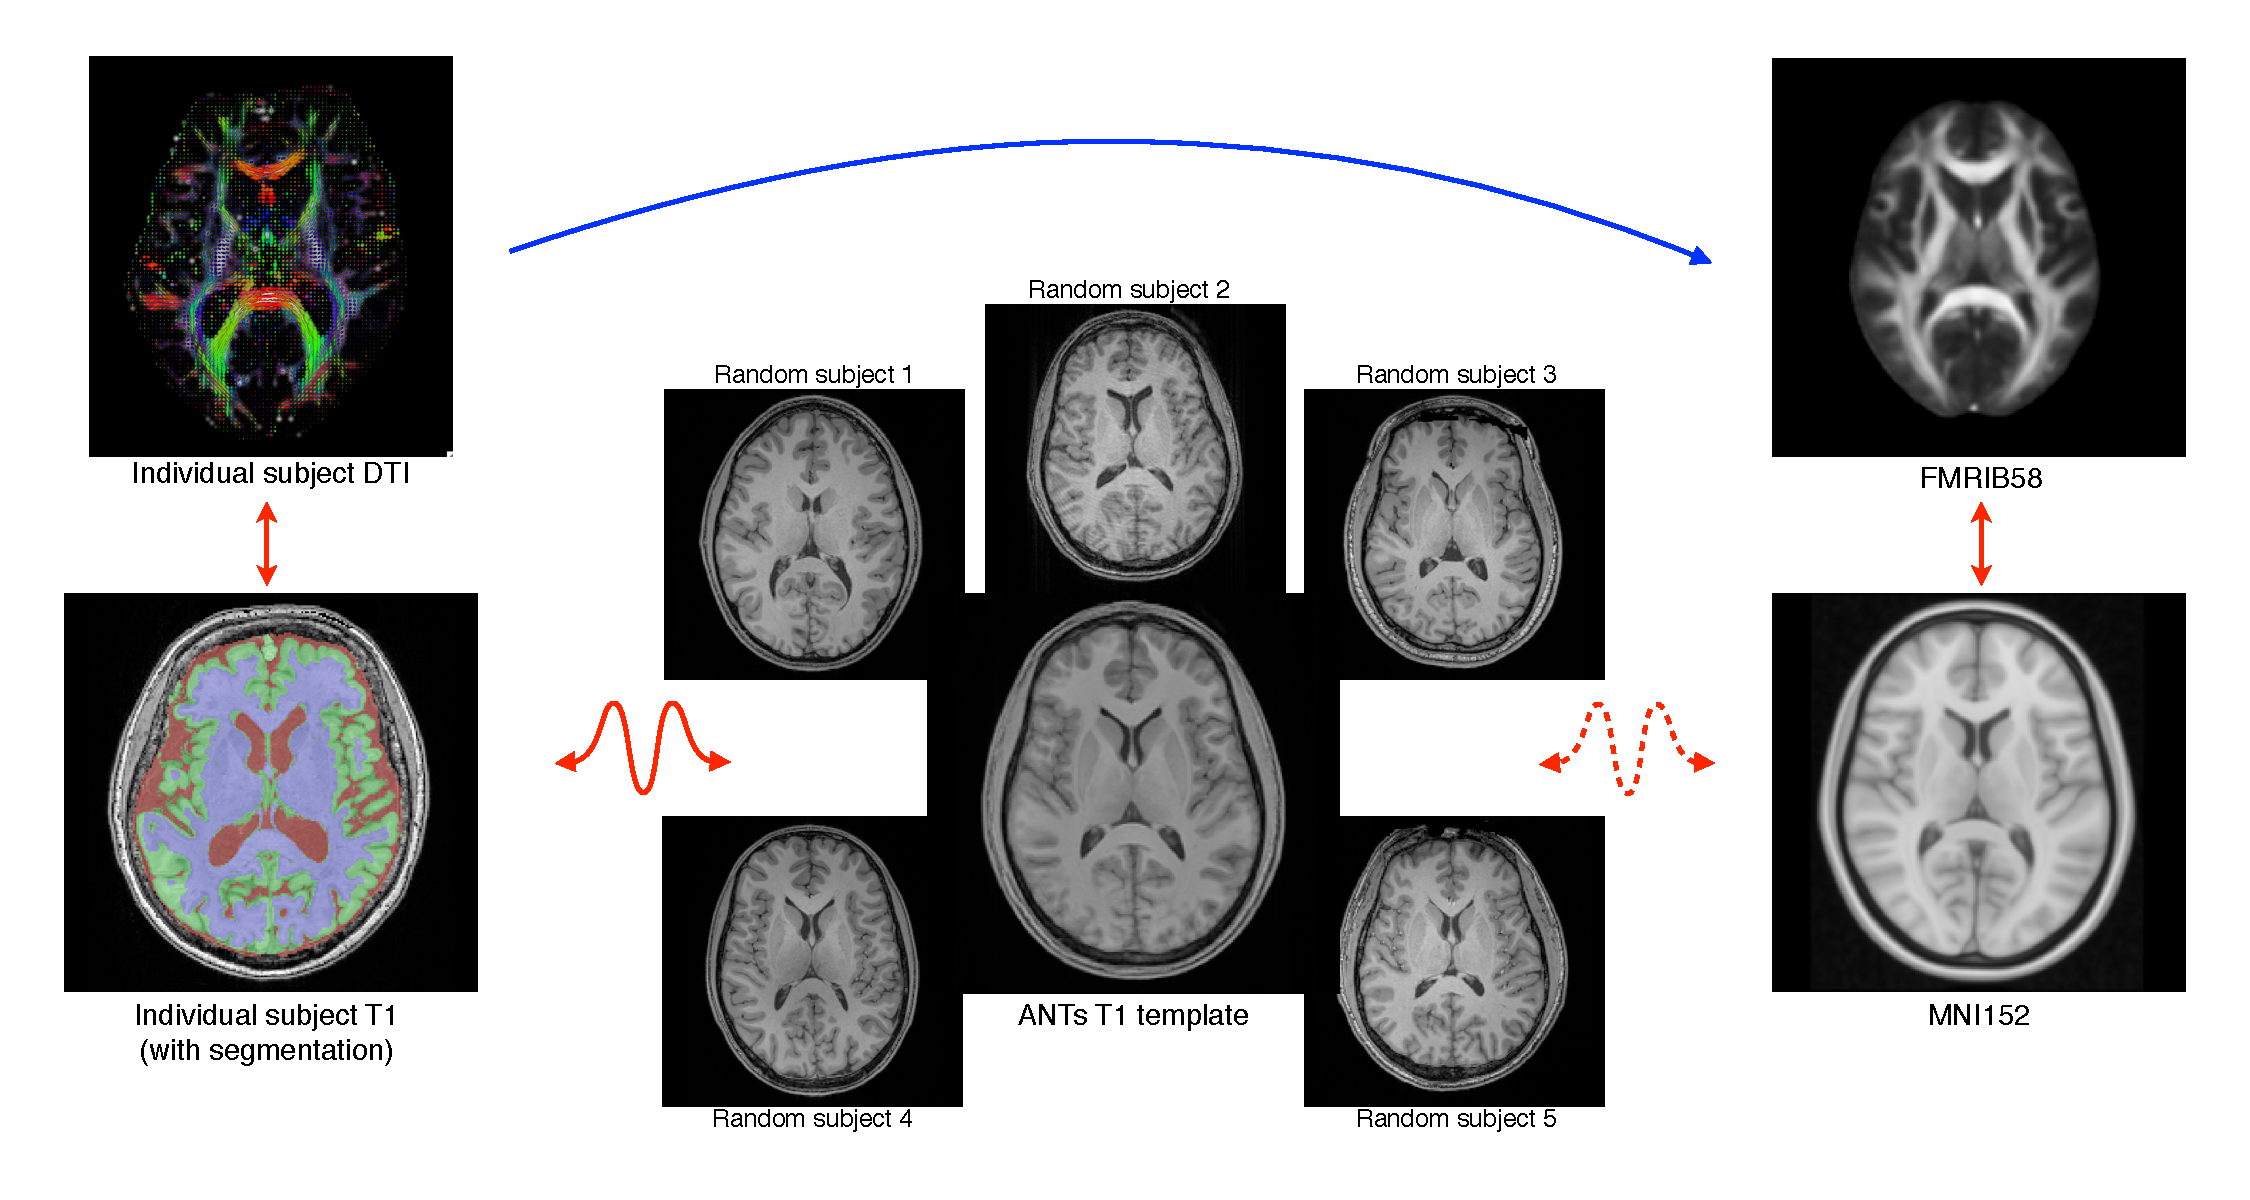
\includegraphics[width=170mm]{workflow.pdf}
\end{tabular}
\caption{Proposed ANTs-TBSS workflow.  In contrast to standard TBSS in which an individual subject's FA is registered to the FMRIB58 template
(transform represented with the blue arrow), our proposed modification first constructs an ANTs optimal anatomical template as illustrated in the center of the figure.  The FA image is then rigidly mapped, with distortion correction, to the individual T1 using the white matter mask as shown on the left.  Each individual T1 is then nonrigidly registered to the anatomical template.  Optionally, one can register the T1 template to the MNI152 template which resides in the same space as the FMRIB58 template.  Thus, the composite transform, carefully constructed without any FA-to-FA image registration, can take an individual subject's FA map (or other DTI-derived measure) to the desired standardized coordinate system.    }
\label{fig:workflow}
\end{figure*}


Prior to the advent of TBSS, voxel-based approaches, such as statistical parametric mapping \cite{Ashburner2000}, were used in assessing voxel-wise population differences \cite{Rugg-Gunn2001,Watkins2001,Kubicki2005,Park2004} using DTI data. In addition to concerns regarding the general application of SPM \cite{Bookstein2001,Ashburner2001,Davatzikos2004}, particularly the requirement for stringent spatial normalization,
issues specific to the application to DTI-derived measures, such as the effects of size variation of the smoothing kernel and the potential non-normality of the residuals \cite{Jones2005}, encourage caution in the application of SPM to DTI-derived data.  Although the latter can be addressed via the use of non-parametric testing \cite{Chung2008}, addressing the former in a principled way is elusive.

It was precisely due to these concerns that the TBSS framework was developed constituting an entire processing pipeline spanning from the reconstruction of the DTI tensorial data
%to the calculation of the corresponding DTI-derived scalar measures (typically fractional anisotropy (FA)), to the nonrigid alignment of the population to a standard coordinate system and skeletonization, and, finally, 
through to the statistical analysis for discerning differences across populations.  Major intermediate steps include the calculation of the corresponding DTI-derived scalar measures (typically fractional anisotropy (FA) \cite{Basser1996}), nonrigid alignment of the population to a standard coordinate system, and subsequent ``skeletonization'' of the mean of the aligned FA maps.  The alignment to a standard space is performed in such a way to remove the smoothing step associated with SPM.  Skeletonization and its projection across all registered DTI-derived scalar images is meant to accommodate the possibility of imperfectly aligned data.  However, as shown in a recent study \cite{Zalesky2011}, although the alignment error is reduced with the skeleton projection step, misalignments still remain post-projection.  Added to this is the potential confounding effect of minimizing data differences via nonrigid registration which are potentially the precise differences to be statistically quantified.

Because spatial normalization is critical to obtaining valid results, we propose a modification of the standard TBSS pipeline directed at some of these residual concerns which we refer to as ANTs-TBSS.  Instead of DTI-derived scalar alignment via the images themselves (either random subject selection or locating an approximation to the ``mean subject'') or to a standard template (e.g. FMRIB58\_FA\_1mm.nii.gz which we denote as ``FMRIB58'' in the remainder of the text), we evaluate the substitution of an anatomical, i.e. T1-weighted, unbiased shape/intensity template constructed from the population images.  DTI-derived images can then be mapped to their corresponding T1-weighted image in a highly constrained manner and subsequently mapped to the template via nonrigid registration of the T1-weighted image.  This eliminates any possible complications associated with direct FA-to-FA image registration.


We recognize that using the anatomical images in the alignment process has been previously proposed (in fact, such a suggestion occurs in the {\it Future directions} section of the original TBSS paper).  Our contribution stems from the specific proposal of using a high performance \cite{Klein2009}, nonrigid registration algorithm \cite{Avants2011}, which forms the underlying machinery for an optimal template construction algorithm \cite{Avants2010}, in facilitating alignment between DTI-derived scalar images for cross-population studies.  This results in a few advantages in using ANTs-TBSS vs standard TBSS:
\begin{itemize}
\item As explained in \cite{Avants2010}, ANTs optimal template construction creates a true Frech\'et mean from the population sample with high resolution which facilitates within-group registration.  This obviates the need for an externally-derived template or an $\OO{n^2}$ search for an approximation to the mean subject or the bias resulting from random subject selection.
\item Since the creation of the standardized coordinate system is performed using the anatomical images, nonrigid registration of the DTI-derived scalar images is 
minimized thus mitigating the confounds described previously.  Each DTI-based image is rigidly registered to its corresponding T1 image followed by a small number of nonrigid registration iterations to account for echo planar imaging (EPI) distortion \cite{Wu2008}.  
\item Although ANTs-TBSS increases the total number of registrations to be performed, this makes the composite registration between an individual DTI-derived image to the template more robust as the shape distance between registrations is minimized.
\item Instead of Gaussian smoothing as with SPM, TBSS uses the warping process to FMRIB58 by default to provide an indirect smoothing.  Such resampling occurs in ANTs-TBSS as a by-product of the registration of the DTI-derived image to the corresponding T1 image in a subject-specific manner.
%\item Instead of using thresholding to create the white matter segmentation from which the skeleton is created, an anatomically-based segmentation, either in the template space or in each subject space followed by a label fusion technique (e.g. majority voting), can be used to ultimately provide a more accurate skeleton.
\item Oftentimes TBSS is only one of several neuroimage analyses performed in a population-based study.  Other investigations, such as voxel- and tensor-based morphometry, cortical thickness measurements, etc. can take advantage of the anatomical template used in ANTs-TBSS.
\end{itemize}


Of practical significance, we note that all software components described in this paper, similar to FMRIB's software library (FSL), of which TBSS is a component, are publicly available as open source primarily through the Advanced Normalization Tools (ANTs) repository.%
\footnote{
http://www.picsl.upenn.edu/ANTs
}
In addition to registration and template building, ANTs also includes brain extraction \cite{Avants2010a}, bias correction \cite{Tustison2010}, $n$-tissue segmentation \cite{Avants2011a}, and cortical thickness estimation solutions \cite{Das2009}.  %As part of this work, we also explicitly show how one can merge the ANTs and TBSS components into a single modified ANTs-flavored TBSS pipeline.
\begin{figure}
\begin{tabular}{c}
  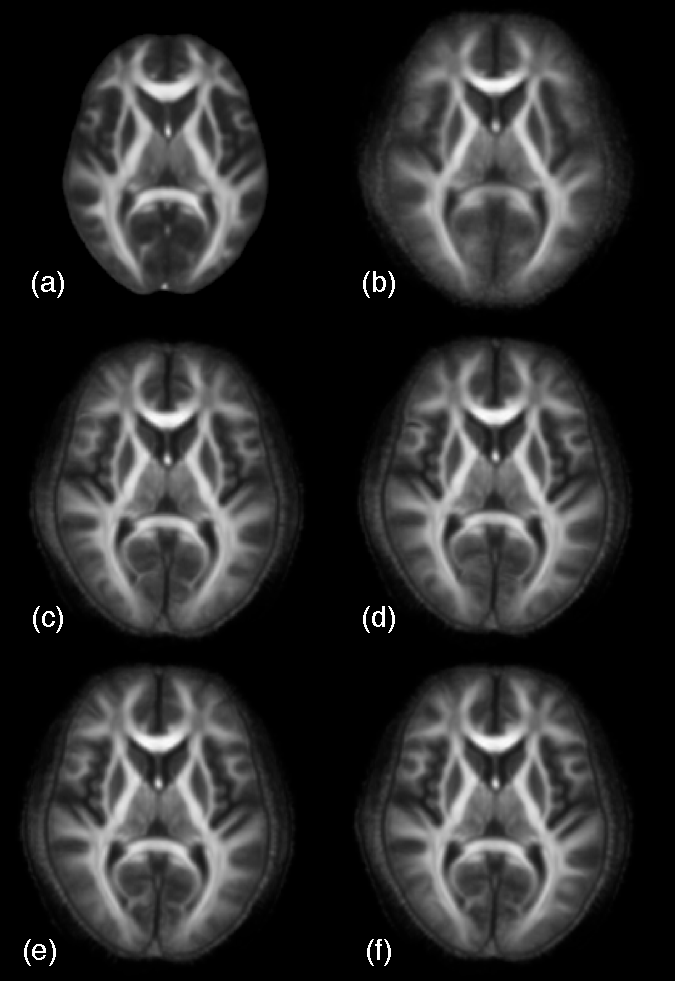
\includegraphics[width=80mm]{NKI.pdf}
\end{tabular}
\caption{Axial slice 80 of FA mean images used in the NKI alignment assessment.  (a) The standard FMRIB58 template. (b) The mean FA image of all aligned 57 NKI data using the TBSS default FLIRT/FNIRT parameters optimized for registration to (a).  
(c)-(f) The mean FA image produced using the ANTs template-based strategy employing 5, 10, 20, and 30 randomly chosen subjects, respectively, warped to the space of (a).  Note the visual alignment difference particularly in the peripheral white matter complex.
}
\label{fig:NKI}
\end{figure}


We first describe in greater detail the proposed ANTs-TBSS framework with an emphasis on comparison with standard TBSS.  We then describe the two open data sets used to evaluate the proposed methodology in addition to a description of diffuse TBI data 
also used to illustrate concepts discussed in this work.
%and analysis previously reported in \cite{Avants2008}.   
%The complementary assessment performed in this paper is used to provide additional analyses to these previous findings.

%A crucial component of TBSS is the alignment of the DTI-derived scalar images \cite{Zalesky2011}. 
%
%Voxel-based morphometry vs. tractography vs. tract-specific analysis
%
%Talk about {\em skeleton projection} and how our work is different from \cite{Zalesky2011}.
%Also talk about the advantages over building a dti-based template as discussed in 
%\cite{Hecke2010}.



\section{Material and Methods}

%In order to understand the differences in approaches, we first briefly describe
%the current TBSS protocol as it is implemented.  This is followed by a
%brief outline of the proposed modification using ANTs.  Afterwards
%we give a description of the data sets used to demonstrate the methods.

\subsection{Tract-Based Spatial Statistics}

FSL hosts a large number of excellent algorithms for computational neuroanalysis.  These include, among others, well-known tools for image segmentation (FAST---\cite{Zhang2001}), linear (FLIRT---\citep{Jenkinson2001}) and nonlinear (FNIRT) image registration, brain extraction (BET---\citep{Smith2002}), as well as TBSS.
For the comparative evaluation studies used in this manuscript, TBSSv1.2%
\footnote{
Build 416 downloaded from the FMRIB web site http://www.fmrib.ox.ac.uk/fsldownloads/ on November 18, 2010.
}
was used.  The actual code pipeline constituting TBSS prior to statistical analysis consists of the following 4 shell scripts:
\begin{description}
  \item[tbss\_1\_preproc]  Input is a directory of FA images which are slightly eroded and then organized into a separate FA directory.  A mask is also generated for each input FA image for use during the spatial normalization process.
  \item[tbss\_2\_reg]  The organized FA data and corresponding masks produced in the previous step are warped to one of three possible coordinate systems using FLIRT/ FNIRT:  1)  the atlas included with the FSL download---FMRIB58---(recommended), 2) a user-specified target image or 3) an exhaustive search for the ``optimal'' target image.  In \cite{Smith2006}, page 1491 section {\it Identifying the target for alignment}, the latter option was advocated based on the observation that average FA images tend to be blurred in contrast to the FA of a single subject.  However, even though it would be faster to simply choose a single subject at random, the complexities of nonrigid image registration would seemingly promote the exhaustive search over random selection.   As a compromise between these two options, the first option in the script is to use FMRIB58 which also resides in the space of the MNI152 T1 template.  It should also be noted that this particular script invokes another FSL script, {\bf fsl\_reg}.  An option associated with {\bf fsl\_reg} permits the use of an FNIRT configuration file which has been optimized for use with the FMRIB58 atlas.  
  \item[tbss\_3\_postreg] The mean FA image is generated from the aligned FA images which is subsequently skeletonized.
  \item[tbss\_4\_prestats] The skeleton mask is created by thresholding the mean FA skeleton.  The skeleton distance map is then generated and all FA data are projected onto the skeleton.
\end{description}

\subsection{ANTs-Flavored TBSS}
\label{sec:ANTs-TBSS}

Our proposed modification to standard TBSS is illustrated in Figure \ref{fig:workflow}.  Instead of direct FA-to-FA registration, our ANTs-based modification can be described as follows:

\begin{enumerate}
  \item Build the anatomical template from  the population sample or sample subset using SyGN.
  \item If only using a sample subset for template creation, warp the remaining
        anatomical data to the template and save the resulting transformation for each         
        subject indexed by $i$ ($T^i_{template}$).
  \item Find the optimal transformation from each
        subject's FA to the anatomical template:
  \begin{enumerate}
  \item For each anatomical image, segment the white matter (in ANTs one can use N4 bias correction and Atropos $n$-tissue segmentation).
  \item Rigidly transform each subject's average DWI to the bias-corrected anatomical
        image ($R^i_{dwi}$).
  \item Perform distortion correction on the FA to anatomical mapping 
        by localized nonrigid registration
        of rigidly transformed FA map ($=R^i_{dwi} \mathrm{FA}$) using
        the white matter mask obtained in step 3(a) ($T^i_{FA}$).
  \item For each subject, concatenate the transforms which maps each
        subject's FA to the template ($T^i_{total} = T^i_{template} \circ 
        T^i_{FA} \circ R^i_{dwi} \mathrm{FA}$).
  \item Warp each subject's FA or MD map to the template using $T^i_{total}$.
  \end{enumerate}      
  \item Perform the remaining portions of the standard TBSS pipeline:
    \begin{enumerate}
      \item Create the mean FA image from all template-aligned FA images.
      \item Produce the white matter skeleton from the mean FA image.
      \item Create skeleton distance map and project all FA data onto the skeleton.
      \item Run the statistical analysis.
    \end{enumerate}
\end{enumerate}

%Provide sufficient detail to allow the work to be reproduced. Methods already published should be indicated by a reference: only relevant modifications should be described.

%\subsection{Symmetric Group Normalization Template Creation}

%Due to the nonlinearity inherent in morphometric neuromaging studies, choice of coordinate
%system can affect quantitative outcome \citep{Thompson2000,Senjen2005}.  
%This dependence has motivated significant work in defining coordinate systems
%using population-derived templates \cite{Joshi2004,Lorenzen2006,Avants2010}. 
%
%based on \cite{Klein2009}
%symmetric group-wise normalization scheme for template co
%
%nstruction was presented in \cite{Avants2010}.  
%
%
%\subsection{Benefits of our approach}
%\begin{itemize}
%   \item White matter segmentations can be performed on the T1 template 
%\end{itemize}
%
%
%\subsection{ANTs-Flavored TBSS}


%\subsection{ANTs-Flavored Tract-Based Spatial Statistics}
%
%\begin{enumerate}
%  \item Create the anatomical template from sample T1 images, i.e.
%\begin{command}
%\lstsetcpp
%\begin{lstlisting}
%$ buildtemplateparallel.sh -d 3 -o T_ -c 0 -g 0.25 -i 4 \
%    -m 50x50x20 -n 1 -r 1 -s CC -t GR T1*.nii.gz
%\end{lstlisting}
%\end{command} 
%\newline
%  where the following flags are used:
%  \begin{description}
%    \item[-d] is the image dimension,
%    \item[-o] is the output prefix where the final template will be named \verb#T_template.nii.gz#,
%    \item[-c] specifies the computational parallelization method,
%    \item[-g] is the gradient step size, 
%    \item[-i] is the number of template-building iterations,
%    \item[-m] is the maximum number of iterations per pairwise registration,
%    \item[-n] is a boolean flag denoting whether or not N4 bias correction is used,
%    \item[-r] is a boolean flag denoting whether or not a rigid registration is used to initialize the template,
%    \item[-s] specifies the similarity metric used (\verb#CC# = cross correlation), and
%    \item[-t] specifies the transformation model used (\verb#GR# = greedy SyN).
%  \end{description}
%The list of files \verb#T1*.nii.gz# denote the set of T1 images used to create the template.  The output consists of the template and the transforms mapping between the subject and template.  Although these parameters generally work quite well, additional information can be found in the help menu of \verb#buildtemplateparallel.sh#.
%\item For each subject, use N4 and Atropos to segment the white matter in each subject's T1 following skull stripping (options include BET \cite{Smith2002} or Atropos \cite{Avants2010a}).  
%\begin{command}
%\lstsetcpp
%\begin{lstlisting}
%$ N4BiasFieldCorrection -d 3 -i T1_subX_brain.nii.gz \
%    -b [200] -c [50x50x50x30,1e-5] \
%    -x T1_subX_mask.nii.gz -o T1_subX_n4.nii.gz
%\end{lstlisting}
%\end{command} 
%\newline
%  where \verb#T1_subX_mask.nii.gz# is the output of the skull stripping step 
%  with brain voxel values of `1' and `0' elsewhere.  The following flags are used:
%  \begin{description}
%    \item[-d] is the image dimension,
%    \item[-i] defines the input image,
%    \item[-b] specifies the ``spline distance'',
%    \item[-c] defines the iterations and convergence threshold, and
%    \item[-o] specifies the output image.
%  \end{description}
%Other options can be explored with the help menu (use \verb#--help#).
%\begin{command}
%\lstsetcpp
%\begin{lstlisting}
%$ Atropos -d 3 -a T1_subX_n4.nii.gz -i kmeans[3] \
%    -m [0.2,1x1x1] -c [5,0.0000001] -k Gaussian \
%    -x T1_subX_mask.nii.gz -o T1_subX_atropos.nii.gz
%\end{lstlisting}
%\end{command} 
%\newline
%  the following flags are used:
%  \begin{description}
%    \item[-d] is the image dimension,
%    \item[-a] defines the input image,
%    \item[-i] specifies the initialization method (here we are using K-means with 3 classes),
%    \item[-m] is the 
%    \item[-c] defines the iterations and convergence threshold, and
%    \item[-o] specifies the output labeled image.
%  \end{description}
%Other options can be explored with the help menu (use \verb#--help#).
%\newline
%This step provides the white matter ma
%\end{enumerate}





\subsection{Imaging Data}

The tensorial data associated with each of the following data sets were reconstructed from the diffusion weighted sequence using Camino%
\footnote{
http://camino.org.uk/
}---an open source toolkit for diffusion MRI processing and analysis \cite{Cook2006} in combination with ANTs-based registration for motion correction of the DTI sequence.

\subsubsection{Data from the International Neuroimaging Data-sharing Initiative (INDI)}

In support of open science, the 1000 Functional Connectomes Project (FCP)%
\footnote{
ttp://fcon\_1000.projects.nitrc.org
} 
was initiated
on December 11, 2009 by various members of the MRI community \cite{Biswal2010}.  Motivated by the absence of neuroimaging data for research, this initiative seeks to form collaborative partnerships with imaging institutions for sharing well-documented multi-modal image sets accompanied by phenotypic data.
Commitments from institutions such as they NYU Institute for Pediatric Neuroscience and the Nathan Kline Institute (NKI)--Rockland have already resulted in prospective data repositories
currently distributed to the public via the Neuroimaging Informatics Tools and Resources Clearinghouse (NITRC).%
\footnote{
http://www.nitrc.org
}
Data from these two institutions were used to demonstrate the alignment properties obtained using SyGN for DTI-derived data normalization.

\paragraph{NKI/Rockland Sample}
Data from the first 14 weeks of prospective data-sharing were downloaded on January 15, 2011 comprised of 74 subjects (average age in years: 32.4 $\pm$ 17.8).  
Due to various technical issues (e.g. lack of corresponding T1 image, failed DTI reconstruction, and inadequate FSL registration performance) only 57 subjects of the NKI data set were used in the image alignment assessment.  
Germane to our evaluation, each imaging session for each subject produced a 64-directional diffusion tensor imaging scan (parameters: conventional single-shot spin echo
EPI pulse sequence, TR = 10000 ms, TE = 91 ms, axial acquisition, 
voxel size = $2 \times 2 \times 2$ mm$^3$) and a T1 anatomical scan (parameters:  TR = 2500 ms, b = 1000 s/mm$^2$ for each direction, 58 contiguous slices of 2.0 mm thickness,
TI = 1200 ms, TE = 3.5 ms, flip angle = 8$^\circ$, 192 contiguous slices of 
1.0 mm thickness, FOV = 256 $\times$ 256 mm$^2$, and voxel size = 1 mm$^3$).  Images were anonymized including defacing of the T1 images prior to upload. 

\paragraph{NYU Institute for Pediatric Neuroscience Sample}
Data from the first 3 parts of prospective data-sharing from NYU were also downloaded on January 15, 2011 comprised of 49 subjects (average age in years: 30.29 $\pm$ 8.81).  All subjects were used in the image alignment assessment.  Two 64-directional DTI scans were performed (parameters: conventional single-shot spin echo
EPI pulse sequence, TR = 5200 ms, TE = 78 ms, axial acquisition, 
voxel size = $3 \times 3 \times 3$ mm$^3$) and a T1 anatomical scan (parameters:  TR = 2530 ms, TE = 3.25 ms, flip angle = 7$^\circ$, 256 contiguous slices of 1.33 mm, FOV = 256 $\times$ 256 mm$^2$, and voxel size = 1.3 mm$^3$).  Images were anonymized including defacing of the T1 images prior to upload. 

%
%The 1000 Functional Connectomes Project (FCP)%
%\footnote{
%http://fcon\_1000.projects.nitrc.org/index.html
%}
%
%{\color{red}{Quote}}  INDI is a next-generation data-sharing effort, with the goal of sharing phenotypically rich imaging datasets, on both retrospective and prospective bases. On 10/8/10, the Nathan Kline Institute (NKI) / Rockland Sample led the way for INDI-Prospective, starting weekly uploads of 5-7 subjects / week (R-fMRI, DTI, and extensive psychiatric and cognitive phenotypic data, including IQ), which continue to progress (currently n = 55 and growing!). More recently, the NYU Institute Pediatric Neuroscience released its sample examining cocaine dependence in adults via INDI-Retro. The list of sites pledging data from around the world is growing, and we are working to generate common phenotypic variables across datasets as possible (notice the frequency with which IQ is starting to appear � it�s just one of our targets!). 
%
%\subsubsection{Nathan Kline Institute (NKI) / Rockland Sample}
%
%{\color{red}{Quote}}  The NKI/Rockland Sample is intended to be a phenotypically rich neuroimaging sample, consisting of data obtained from individuals between the ages of 6 and 85 year-old. All individuals to be included in the sample undergo semi-structured diagnostic psychiatric interviews, and complete a battery of psychiatric, cognitive and behavioral assessments in order to provide comprehensive phenotypic information for the purpose of exploring brain/behavior relationships.
%
%Each subject consists of the following data:
%\begin{itemize}
%\item 10 minute resting state fMRI scan (R-fMRI) 
%\item 6-direction diffusion tensor imaging (DTI) scan 
%\item 64-direction diffusion tensor imaging scan (2mm isotropic)
%\item MPRAGE anatomical scan
%\item A variety of psychiatric, cognitive and behavioral assessments
%\end{itemize}
%
%\subsubsection{NYU Institute for Pediatric Neuroscience}
%
%{\color{red}{Quote}}  Summary: The NYU Phyllis Green and Randolph C?wen Institute for Pediatric Neuroscience (IPN) sample will be a collection of past and present scans obtained from psychiatrically screened individuals ranging in age from 6 to 55 years old. The initial release consists of datasets from 49 psychiatrically neurotypical adults, with age, gender and intelligence quotient (IQ) information provided. Future releases will include more comprehensive phenotypic information, and child and adolescent datasets, as well as individuals from clinical populations.
%
%Each subject consists of the following data:
%\begin{itemize}
%\item At least one 6-minute resting state fMRI scan (R-fMRI)%
%\footnote{
% Most participants have 2 R-fMRI scans, collected less than 1 hour apart in the same scanning session. Rest$_1$ is always collected first.
%}
%\item One high-resolution T1-weighted mprage, defaced to protect patient confidentiality
%\item Two 64-direction diffusion tensor imaging scans
%\item Demographic information (age, gender) and IQ-measures (Verbal, Performance, and Composite; Weschler Abbreviated Scale of Intelligence [WASI])
%\end{itemize}
%
\subsubsection{Diffuse Traumatic Brain Injury Data}

A third data set was obtained as port of a larger effort investigating the relationship between various neuroimaging indices and cognitive and functional abilities in long-term survivors of TBI (principal investigator: John Whyte). A more detailed data description can be found in \cite{Avants2008}. The following is a brief description relevant to our particular study.  
17 controls and 16 patients with TBI were used for the analysis presented in this
work.  Each patient had a history of non-penetrating traumatic brain injury 
of at least moderate severity defined by significant and well-documented
loss or alteration of consciousness following injury in addition to meeting
several other exclusionary criteria.  The healthy volunteers were matched in terms of age, gender, ethnicity, handedness, and
years of education.
High resolution T1-weighted anatomic images were obtained using 3D MP-RAGE 
imaging sequence using the following acquisition parameters: TR = 1620 ms, 
TI = 950 ms, TE = 3 ms, flip angle = 15$^\circ$, 160 contiguous slices of 
1.0 mm thickness, FOV = 192 $\times$ 256 mm$^2$, matrix = 192 $\times$ 256, 
1NEX with a scan time of 6 minutes, and voxel size = 1 mm$^3$.  30-directional
DTI images were also obtained 

%
%\subsubsection{Participants}
%{\color{red}{Quote:}} The data were collected as part of a larger study investigating the neural correlates of attention deficits and treatment responses of various psychoactive drugs in the survivors of TBI (principal investigator: J.W.). Thirty individuals with TBI and 20 healthy volunteers were recruited. We planned to recruit more TBI participants because data of TBI survivors are more likely to be discarded in a typical functional neuroimaging study due to movements in the scanner and poor behavioral performance. TBI participants were recruited from a variety of clinical services at MossRehab and through a consent-based registry of individuals with TBI who are interested in participating in rehabilitation research. To be included, participants had to be between the ages of 16 and 60, and to have a history of non-penetrating traumatic brain injury of at least moderate severity at least 3 months prior to enrollment. Severity level was defined by significant and well-documented loss or alteration of consciousness following injury (i.e., lowest Glasgow Coma Scale (GCS) score of less than 12, or prospectively documented post-traumatic amnesia (PTA) of greater than 1 hour), or focal abnormality on a neuroimaging study that was attributable to traumatic injury. A subjective complaint of attention difficulties by the participant, treating clinician, or caregiver was also required. Potential participants were excluded if they had a history of prem orbid neurologic disease, psychosis, major affective disorder, mental retardation, Attention Deficit Hyperactivity Disorder, or if they were currently abusing alcohol or recreational drugs. Persons who were taking psychoactive medications other than anticonvulsants were also excluded. Participants and/or their involved caregivers (depending on the participant�s cognitive capacity) provided informed consent. The study protocol was approved by the Albert Einstein Healthcare Network and the University of Pennsylvania IRBs. Twenty healthy volunteers, matched to patients for age, gender, handedness, years of education, and ethnicity, participated in the study. Control participants were recruited based on the same inclusion/exclusion criteria as patients, with the exception that they never had a TBI resulting in loss or alteration of consciousness, nor suffered attention complaints. Control participants were recruited through the family and friendship networks of the participants with TBI, and through public advertising.
%Data from one TBI participant whose MRI scan showed a large area of encephalom alacia over almost the entire right hemisphere were excluded. The remaining 29 subjects with TBI included 21 men and 8 women aged between 18 and 58 years (mean age = 36.9, SD = 11.4) with a mean education of 13.1 years (SD = 2.8). Twenty three of them were right-handed (Edinburgh Handedness Inventory, Oldfield, 1971). Fourteen of them were Caucasians, 10 African Americans, 4 Hispanics, and 1 Asian. Selected demographic and clinical characteristics of the TBI survivors are reported in Table 1. Control participants included 17 men and 3 women aged between 21 and 50 years (mean age = 34.9, SD = 9.8) with a mean education of 13.1 years (SD = 1.7). Sixteen of them were right-handed. Eleven of them were Caucasians, 7 African Americans, 1 Asian, and 1 unknown. The two groups did not differ significantly in terms of age, gender, ethnicity, handedness or years of education (tested with t-test or Fisher�s exact test, as appropriate).
%
%\subsubsection{Image acquisition}
%The functional imaging was conducted on a Siemens 3.0 T Trio whole-body scanner (Siemens AG, Erlangen, Germany), using a standard Transmit/Receive head coil. High resolution T1-weighted anatomic images were obtained using 3D M PRAGE imaging sequence using the following acquisition parameters: TR = 1620 ms, TI = 950 ms, TE = 3 ms, flip angle = 15$^\circ$, 160 contiguous slices of 1.0 mm thickness, FOV = 192 $\times$ 256 mm$^2$, matrix = 192 $\times$ 256, 1NEX with a scan time of 6 minutes. The resulting voxel size was 1 mm$^3$.
%Lesion assessment
%To quantify the volume of lesions, a trained observer (J.P.) manually segmented the lesion area under supervision of a neurologist (H.B.C.) with extensive experience in lesion assessment. Focal lesions included any cystic cavities and other focal regions of abnormal signal in the white or gray matter. The ITK-SNAP software \citep{Yushkevich2006} was used for a 3D-based segmentation. Total lesion volume was calculated using a stand-alone utility provided by VoxBo software (Center for Functional Neuroimaging, Philadelphia, PA, http://www.voxbo.org).




\section{Results and Discussion}
%Results should be clear and concise.


\subsection{Alignment Assessment of the INDI Data}

\begin{table}
  \caption{Volume (in voxels) of thresholded mean FA skeletons.}
  \label{table:vol}
  \begin{tabular*}{88mm}{@{\extracolsep{\fill}} ccccc}
  \hline
  {} & \multicolumn{2}{c}{NKI} & \multicolumn{2}{c}{NYU} \\
  \cline{2-5}
  {} & inner & outer & inner & outer \\
  \hline
  FMRIB & 84899 & 122306 & 72765 & 76769 \\
  ANTs$_5$ & 87572 & 134421 & 73650 & 94177 \\
  ANTs$_{10}$ & 86908 & 130569 & 73419 & 98014 \\
  ANTs$_{20}$ & 86523 & 129729 & 73577 & 95484 \\
  ANTs$_{30}$ & 86971 & 128892 & 73443 & 94862 \\
  \hline
  \hline
  \end{tabular*}
\end{table} 

\begin{table}
  \caption{Number of connected components of thresholded mean FA skeletons.}
  \label{table:cc}
  \begin{tabular*}{88mm}{@{\extracolsep{\fill}} ccccc}
  \hline
  {} & \multicolumn{2}{c}{NKI} & \multicolumn{2}{c}{NYU} \\
  \cline{2-5}
  {} & $\geq$ 1 voxel & $\geq$ 2 voxels & $\geq$ 1 voxel & $\geq$ 2 voxels \\
  \hline
  FMRIB & 4340 & 1802 & 2431 & 993 \\
  ANTs$_5$ & 3561 & 1384 & 2278 & 916 \\
  ANTs$_{10}$ & 3413 & 1302 & 2232 & 899 \\
  ANTs$_{20}$ & 3283 & 1252 & 2093 & 885 \\
  ANTs$_{30}$ & 3114 & 1243 & 2128 & 867 \\
  \hline
  \hline
  \end{tabular*}
\end{table} 


Since our proposed modification of TBSS impacts strictly the
critical alignment step, the first set of evaluations demonstrates
the difference between the two methods, i.e. spatial normalization 
via registration of the FA maps to the FMRIB58 template
or spatial normalization via ANTs template construction.  It is important to note that we did not consider normalization either to a random subject
or to the subject best representative of the mean as defined in 
\cite{Smith2006}. The former was not investigated due to the possible bias
in selecting a random subject as described in \cite{Smith2006}.  
Neither was the latter option pursued due to the computational complexity
required for such an $\OO{n^2}$ search over the relatively large NKI and NYU data sets.  In addition, normalization to
the FMRIB58 template is both the default and recommended option
with the parameters of FNIRT optimally tuned for said option.  To warp the MD images following FA registration we used FSL's {\bf applywarp} function using the FA-derived transform. 

%\begin{figure}
%\begin{tabular}{c}
%  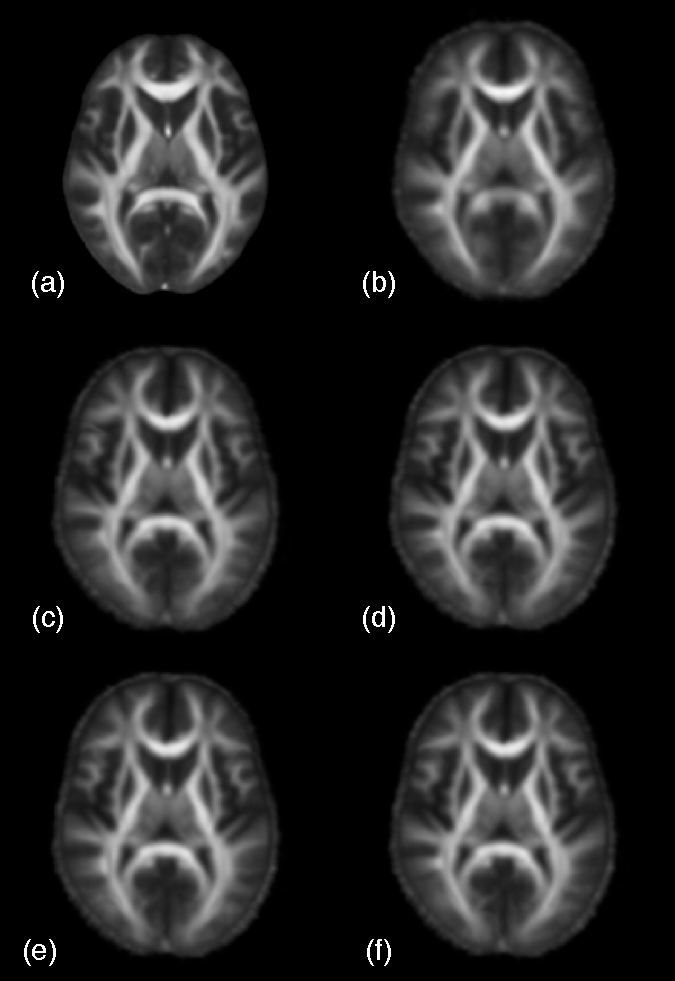
\includegraphics[width=80mm]{NYU.pdf}
%\end{tabular}
%\caption{Axial slice 80 of FA mean images used in the NYU alignment assessment.  (a) The standard FMRIB58\_FA\_1mm template. (b) The mean FA image of all aligned 57 NKI data using the TBSS default FLIRT/FNIRT parameters optimized for registration to (a).  
%(c)-(f) The mean FA image produced using the ANTs template-based strategy employing 5, 10, 20, and 30 randomly chosen subjects, respectively, warped to the space of (a).  Note the visual alignment difference particularly in the peripheral white matter complex.
%}
%\label{fig:NYU}
%\end{figure}



To explore alignment with ANTs-TBSS, 4 templates were constructed for each of the 2 data sets.  Each within-group template was generated from $\{5,10,20,30\}$ randomly selected subjects to see if the number of subjects comprising the template affected the alignment performance. In addition
to the composite transforms described in Section \ref{sec:ANTs-TBSS} to take each subject's FA or MD image to the population-specific anatomical template, we also registered
each ANTs T1 template to the MNI152 template.  This permitted a
standard space for qualitative and quantitative comparison.  


Sample axial slices for all resulting FA mean images for the NKI data set are provided in Figure \ref{fig:NKI}.  We also include the same axial slice of the FMRIB58 template in Figure \ref{fig:NKI} (a) for comparison.  In both sets of sample slices, visual inspection would seemingly indicate better performance with the ANTs-based FA mean images compared with the standard TBSS-produced FA mean image.  Also, there is little discernible difference between the different ANTs results.  Alignment differences between the two approaches are particularly apparent in the peripheral white matter where the anatomical structure in the ANTs template-based FA mean images is visually differentiable.

Relative performance is quantified in the plots produced in Figure \ref{fig:NKIplots} and Figure \ref{fig:NYUplots}.  For both data sets, the mean FA image derived from the standard TBSS approach was thresholded at FA $\geq 0.2$.  These two binary masks obtained in both the NKI and NYU cohorts provided the standard group masks for fair comparisons for all evaluations.    For the aligned images the coefficient of variation (CoV) was calculated in a voxel-wise fashion within the mask.  Intuitively, one would expect a smaller variance across better aligned sets of voxel values thus producing a lower CoV for a given mean value.  By calculating the cumulative distribution function (CDF) of the set of CoV values within the mask, quantitative assessment of alignment performance can be visualized.  In addition to producing CDF plots for voxels within the entire brain mask, we separated the brain into inner and outer sections to investigate the alignment difference between these two regions.  This division was accomplished by applying a distance transform \cite{Maurer2003} to the FSL-provided MNI152 brain mask and thresholding the result such that the outer 30 mm form the outer mask and the subtracted binary image forms the inner mask.  Note that only those voxels that were also within the thresholded FA mask were considered in the inner/outer analysis.


There is a visible improvement in alignment for both data sets using the ANTs-based approach over individual subject FA registration to the FMRIB template.  There is little difference between the ANTs results with only a slight trend in improved performance with the larger template subject sample sizes.  This was the case for all three regional CoV calculations for both data sets.  Also, as expected, there is greater misalignment in the outer region versus the inner core of the white matter mask regardless of methodology.  However, the performance tally was the same in both the inner and outer regions as was the case with the entire white matter mask although the disparity in performance was much less for the NYU data set as the NKI data set most likely due to the differences in resolution of the original DTI.

The improvements seen in the CDF plots are also supported by comparative quantities derived from the skeletons of the different mean FA images.  Since the skeletonization process is meant to determine the center of the various white matter tracts \cite{Smith2006}, a greater volume of skeletonization voxels would indicate identification of more centers of white matter tracts.  In addition, as described in \cite{Zalesky2011}, the number of connected components of the white matter skeleton is directly related to the contiguity and thus inversely related to the level of structure.  Table \ref{table:vol} provides the volume of the mean FA skeletons (thresholded at FA $\geq 0.2$) for standard TBSS protocol using the FMRIB template and the ANTs approach using the various templates.  In agreement with the CDF plots illustrating improved alignment with ANTs, the voxel volumes of the skeletons are greater using ANTs templates with the greatest difference seen in the outer portion of the white matter.
Related, in Table \ref{table:cc}, we provide the number of connected components for both data sets for all isolated components greater in size than 1 voxel and 2 voxels.  Even though the skeletal volumes associated with the ANTs approach are greater, the number of connected components is less which would also support the observation of improved alignment.

 
 
%\begin{figure}
%\begin{tabular}{c}
%  \includegraphics[width=80mm]{inner.png}
%\end{tabular}
%\caption{
%}
%\label{fig:inner}
%\end{figure}
%
%\begin{figure}
%\begin{tabular}{c}
%  \includegraphics[width=80mm]{outer.png}
%\end{tabular}
%\caption{Three-canonical view of the inner
%}
%\label{fig:outer}
%\end{figure}

\begin{figure*}
\begin{tabular}{c}
  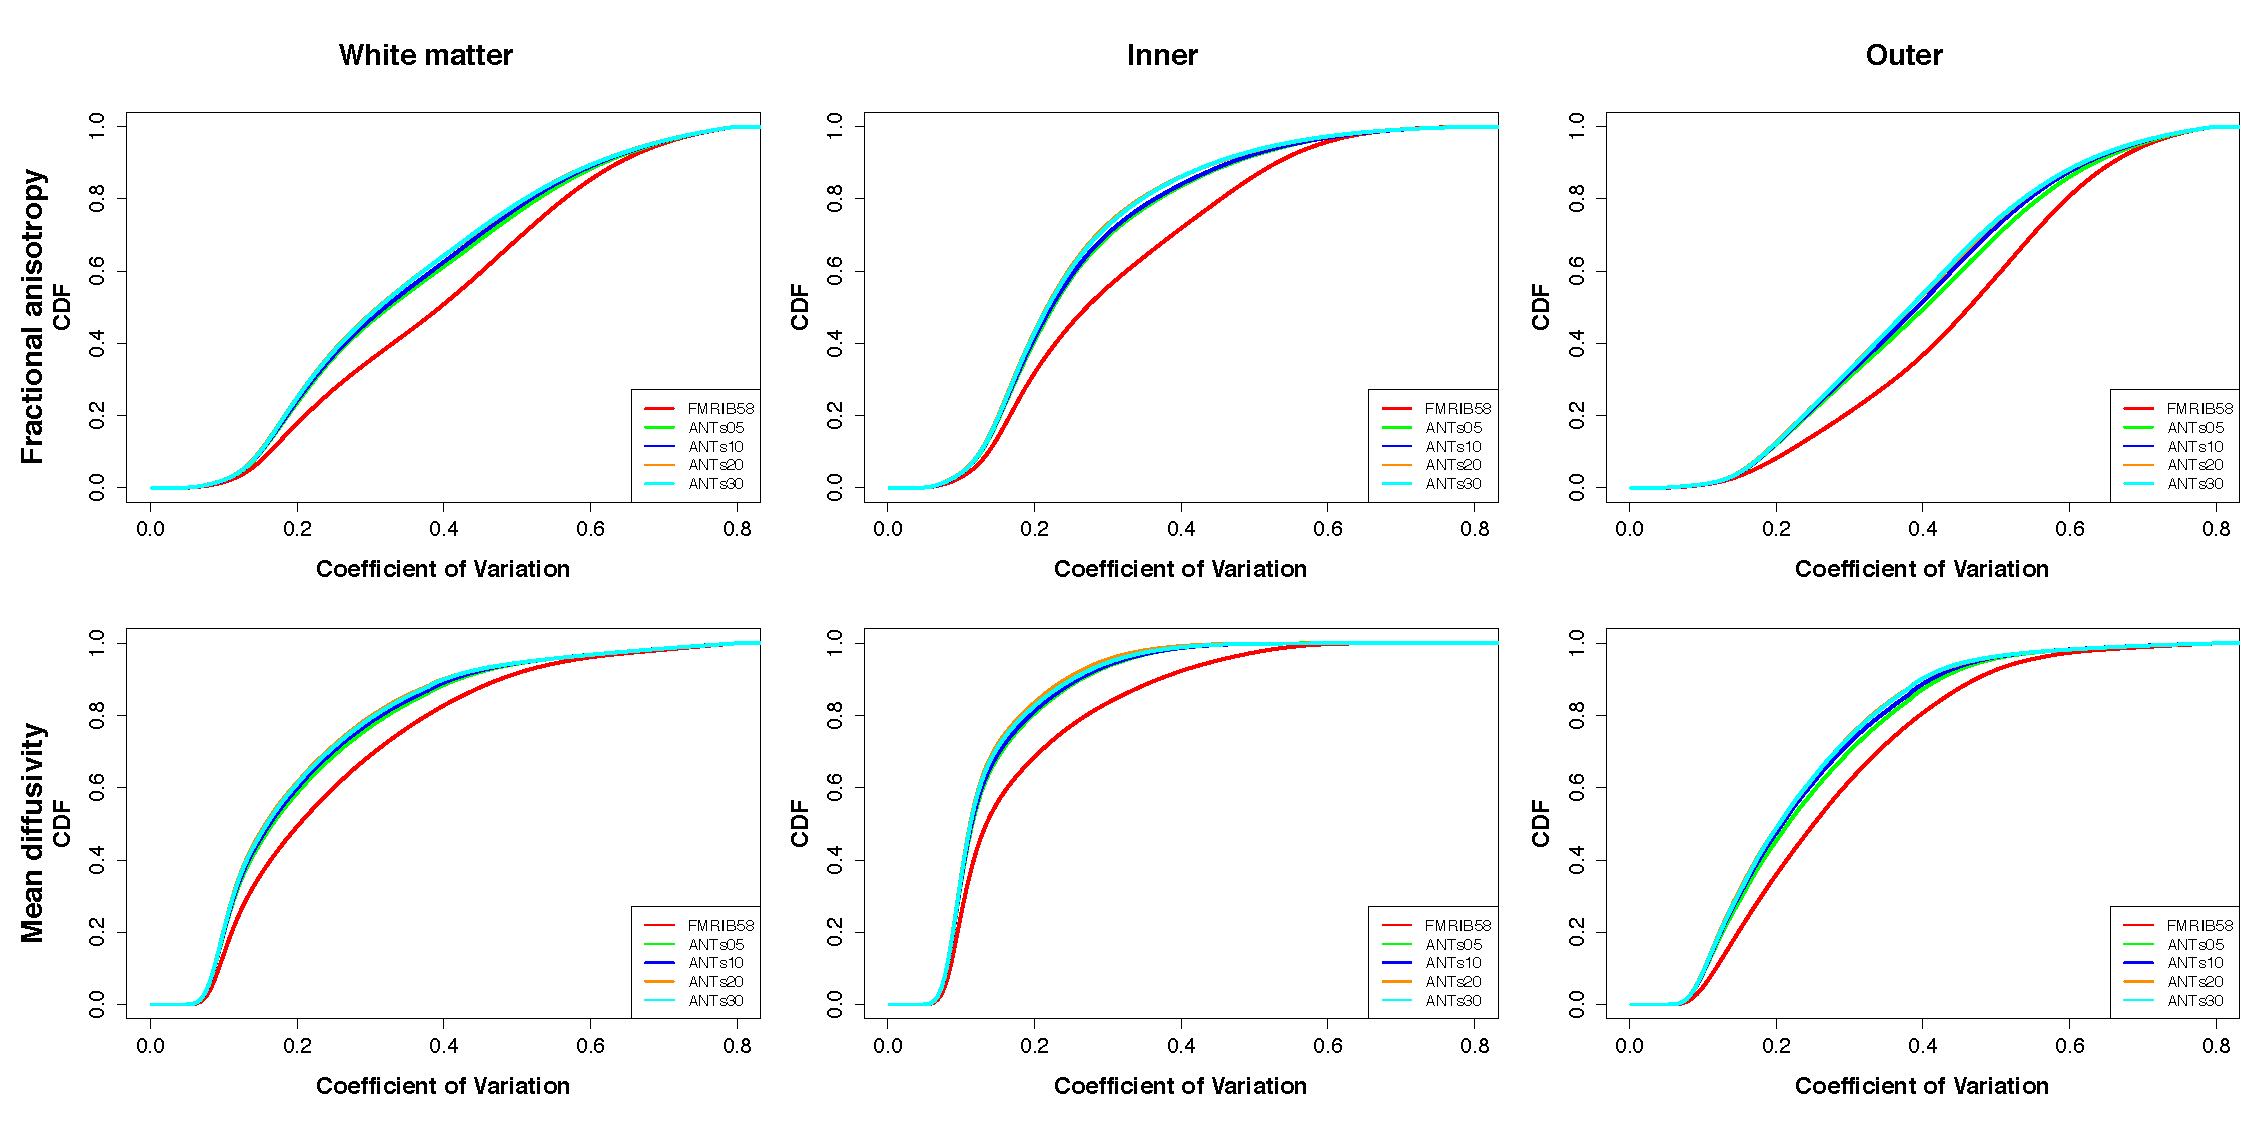
\includegraphics[width=180mm]{NKIplots2.pdf}
\end{tabular}
\caption{{\bf NKI alignment assessment:}  To compare alignments between the  standard TBSS approach of using the FMRIB58 template versus using the different ANTs templates, we calculated the coefficient of variation at each voxel (for both FA and MD) and plotted the CDF over the range of values $[0,0.8]$ accumulated over all the voxels inside the thresholded (FA $\geq 0.2$) standard TBSS mean FA image (see Figure \ref{fig:NKI}(b)).  In addition to the whole brain analysis (first column), the coefficient of variation was separately calculated over the inner and outer portions of the white matter (second and third columns, respectively).  The CDF plots for the ANTs templates are all very similar (although trending towards slight improvement with larger template sample size) and illustrate the general improvement in FA and MD alignment over registration of each FA image to the FMRIB58 template.
}
\label{fig:NKIplots}
\end{figure*}

\begin{figure*}
\begin{tabular}{c}
  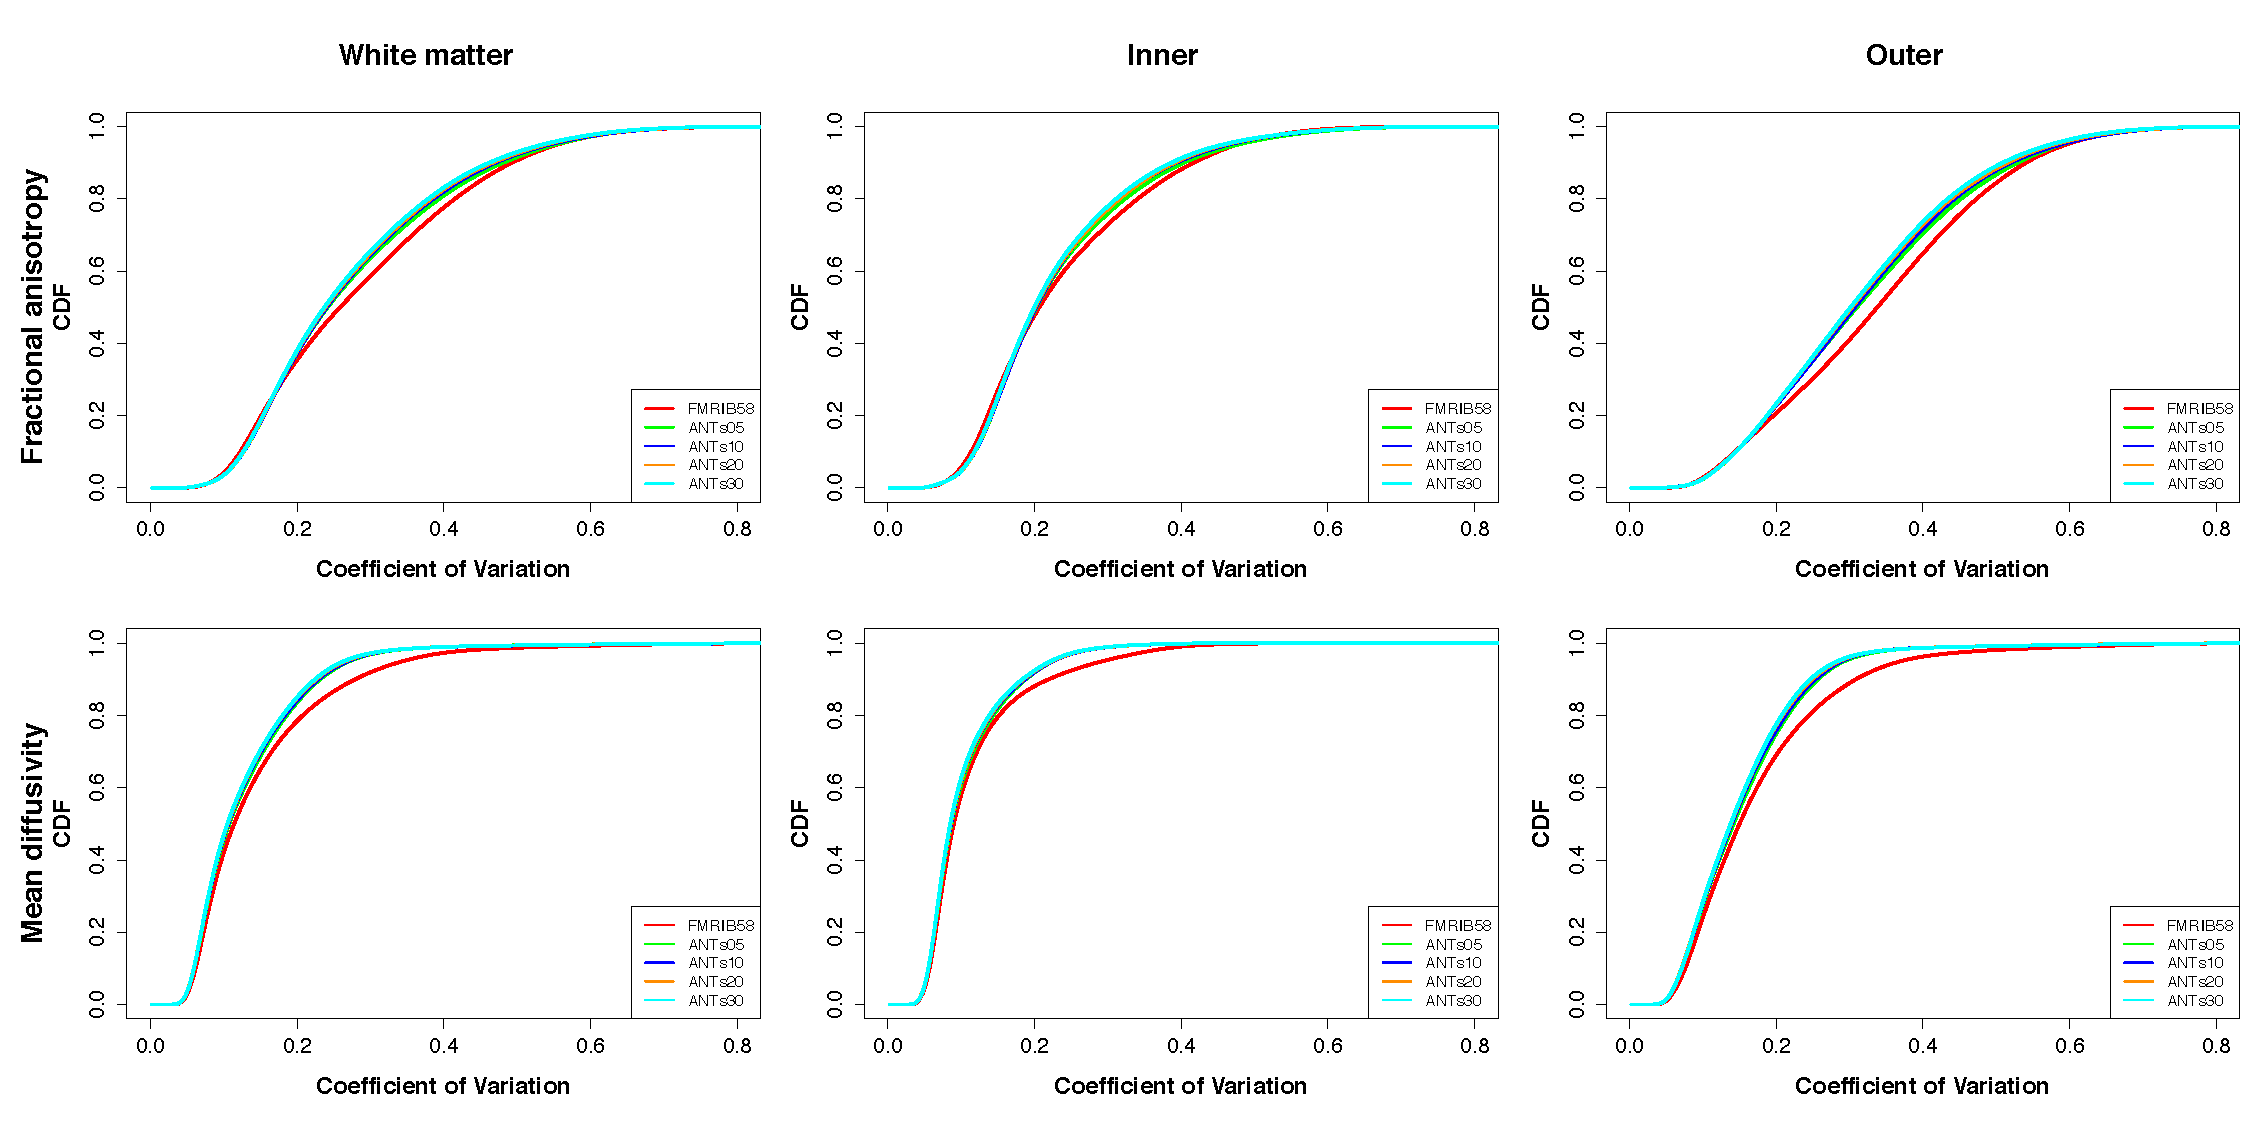
\includegraphics[width=180mm]{NYUplots2.pdf}
\end{tabular}
\caption{{\bf NYU alignment assessment:}  To compare alignments between the  standard TBSS approach of using the FMRIB58 template versus using the different ANTs templates, we calculated the coefficient of variation at each voxel (for both FA and MD) and plotted the CDF over the range of values $[0,0.8]$ accumulated over all the voxels inside the thresholded (FA $\geq 0.2$) standard TBSS mean FA image (see Figure \ref{fig:NKI}(b)).  In addition to the whole brain analysis (first column), the coefficient of variation was separately calculated over the inner and outer portions of the white matter (second and third columns, respectively).  The CDF plots for the ANTs templates are all very similar (although trending towards slight improvement with larger template sample size) and illustrate the general improvement in FA and MD alignment over registration of each FA image to the FMRIB58 template.
}
\label{fig:NYUplots}
\end{figure*}



\subsection{TBSS and ANTs-TBSS of TBI Cohort} 

\begin{figure}
\begin{tabular}{c}
  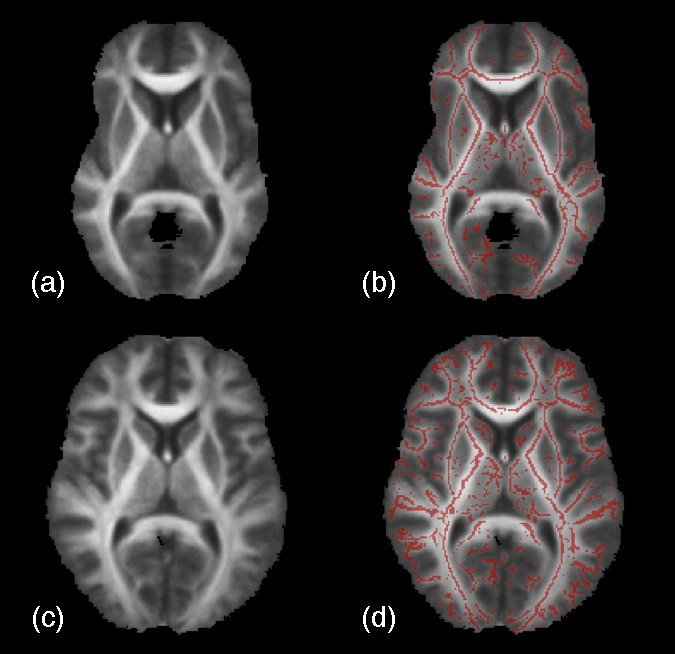
\includegraphics[width=80mm]{meanFA.pdf}
\end{tabular}
\caption{Comparison of mean FA images used in TBSS taken from the TBI data described in Section 2.  The mean FA image illustrated in (a) is created by mapping the sample FA population to the default FMRIB58 template which is the standard protocol for TBSS.  In comparison, the mean template represented in (c) is created from alignment of the population sample to the optimal T1 template as described in the paper. The respective skeleton masks in (b) and (d) are created by thresholding the resulting skeleton values $\geq 0.2$.  The yellow area points to a peripheral difference in findings between the two analyses.
}
\label{fig:meanFA}
\end{figure}

A patient template and a control template were  constructed 
using the ANTs software from all subjects of the respective populations.  These two templates were then used to create a third template which provided the standard space for the ANTs-based TBSS assessment.  Standard TBSS was also performed.  

The resulting mean FA images and thresholded skeletons are represented in Figure \ref{fig:meanFA} which demonstrate appreciable in alignment.  These images support earlier findings in improved alignment with the ANTs-based approach.  The skeleton masks were produced by thresholding the skeleton values at FA $\geq 0.2$ and it would seem that the improved alignment produces a more extensive skeletal network for greater localization testing of significant differences, particularly in the outer white matter regions.  Given that TBSS is intrinsically a statistical method for finding local differences, improved alignment would presumably provide increased regional sensitivity to differences.

%
%Comparison of areas of significant difference between the two groups for both methodologies can be seen on several corresponding axial slices in Figure \ref{fig:hoonData}.  The majority of the areas of significance overlap between the two analyses although the yellow arrow points to one difference situated in the right frontal lobe.  


%As an additional quantitative comparison, we calculated the volumetric ratio between areas of significance and the volumetric brain mask for both $p = 0.01$ and $p = 0.05$.  For standard TBSS, the MNI 152 "first brain mask" was used and for the ANTs template, Atropos was used to obtain a mask by skull stripping of the final template.  These values are given in Table \ref{table:hoon}.
%
%
%\begin{table}
%  \caption{Volumetric ratio differences between ANTsTBSS and TBSS.}
%  \label{table:hoon}
%  \begin{tabular*}{88mm}{@{\extracolsep{\fill}} cccc}
%  \hline
%  {} & $\frac{V(\mathrm{mean\,FA\,mask})}{V(\mathrm{brain\,mask})}$ & $\frac{V(\mathrm{sig.\,areas})}{V(\mathrm{mean\,FA\,mask})}$ & $\frac{V(\mathrm{sig.\,areas})}{V(\mathrm{brain\,mask})}$ \\
%  \hline
%  $p \leq 0.01$ & {} & {} & {} \\
%  $p \leq 0.05$ & {} & {} & {} \\
%  \hline
%  \hline
%  \end{tabular*}
%\end{table} 





%\begin{figure}
%\begin{tabular}{c}
%  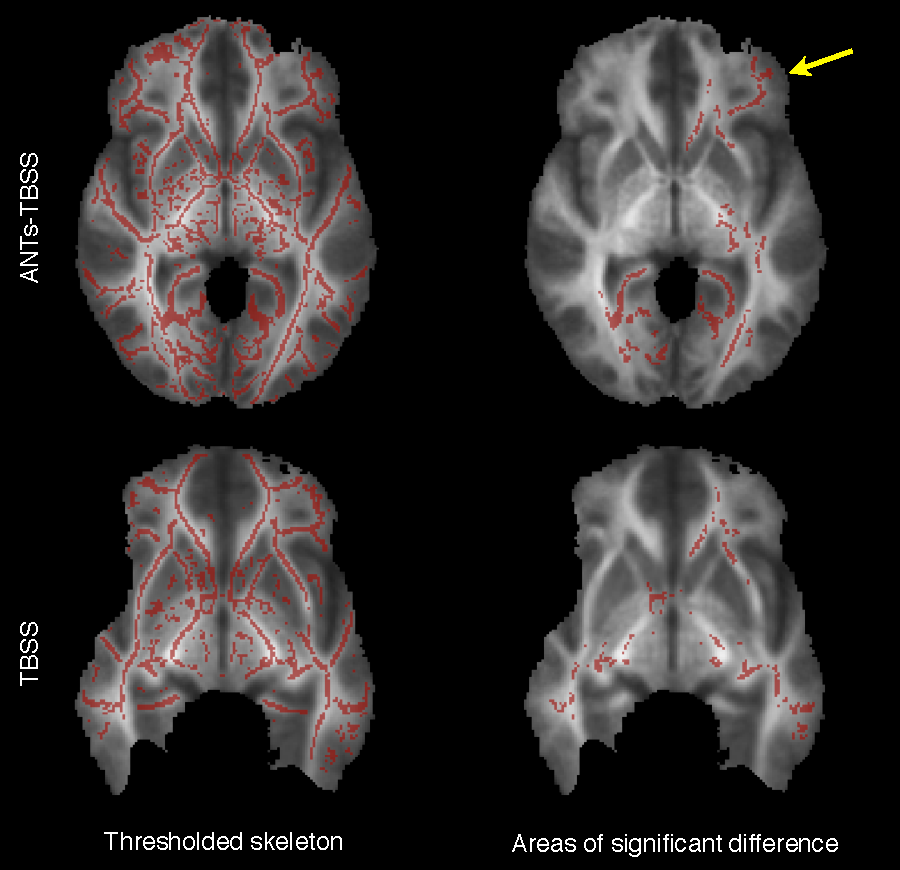
\includegraphics[width=80mm]{hoonData2.pdf}
%\end{tabular}
%\caption{Results of TBSS analysis using both the ANTs template-based approach (top row) and the standard TBSS protocol (bottom row).  Axial slices were chosen based on visual assessment of correspondence in both the ANTs template and MNI 152 template.
%On the left is the thresholded skeleton overlaid on the mean FA image.  
%On the right, significant areas of difference are given in red ($p \leq 0.01$ after the threshold-free cluster enhancement correction described in \cite{Smith2009}).  The yellow arrow points to an area of significant difference in the peripheral white matter found using ANTs-TBSS.
%}
%\label{fig:hoonData}
%\end{figure}





%\section{Discussion}
%This should explore the significance of the results of the work, not repeat them. A combined Results and Discussion section is often appropriate. Avoid extensive citations and discussion of published literature.

\section{Conclusions}
%The main conclusions of the study may be presented in a short Conclusions section, which may stand alone or form a subsection of a Discussion or Results and Discussion section.

The popularity of FSL's TBSS is due, in large part, to its ease of use.  Anybody interested in performing a neuroimaging study in which DTI-derived measures are compared across populations can simply download FSL and immediately apply it to their data.  The proposed work is a substantial improvement to the core TBSS framework which dovetails with FSL.  In addition, it is comparably easy to download and apply what we have proposed in the form of ANTs-TBSS.  




The proposed improvement potentially has many benefits which were listed in the introduction.  Such benefits range from the theoretical in the form of eliminating the confounding effects of registering data which is to be statistically differentiated to the practical---reusing ANTs template construction for other neuroimaging analyses.
In performing the various analyses described in the work, it was pleasantly surprising to discover how well the alignments were for the ANTs template data considering that alignment was based on FA-to-FA correspondence and no such image registrations were performed to align FA directly with FA as with TBSS.  Furthermore, since TBSS is a local quantification method with increased statistical power through the use of the skeletonization and projection step, improved alignments can increase the regional sensitivity to local white matter differences particularly in the peripheral tracts.

%% The Appendices part is started with the command \appendix;
%% appendix sections are then done as normal sections
%% \appendix

%% \section{}
%% \label{}

%% References
%%
%% Following citation commands can be used in the body text:
%% Usage of \cite is as follows:
%%   \cite{key}          ==>>  [#]
%%   \cite[chap. 2]{key} ==>>  [#, chap. 2]
%%   \citet{key}         ==>>  Author [#]

%% References with bibTeX database:

\section*{Acknowledgments}
All visualizations were performed using ITK-SNAP%
\footnote{
http://www.itksnap.org/
}
\cite{Yushkevich2006} and
DTI-TK.%
\footnote{
http://www.nitrc.org/projects/dtitk/
}

\section*{References}

\bibliographystyle{elsarticle-harv}
\bibliography{references}


%% Authors are advised to submit their bibtex database files. They are
%% requested to list a bibtex style file in the manuscript if they do
%% not want to use model1-num-names.bst.

%% References without bibTeX database:

% \begin{thebibliography}{00}

%% \bibitem must have the following form:
%%   \bibitem{key}...
%%

% \bibitem{}

% \end{thebibliography}


\end{document}

%%
%% End of file `elsarticle-template-1-num.tex'.
